\section{From renewal pieces to the unrestricted thermal law}\label{R:sec:thermal}
We now prove the full-plane thermal assertion. The proof separates three tasks: identify the half-plane remainder, construct a recoverable family giving the plane denominator, and control paths whose endpoints have small vertical separation. The geometric estimate used in the last task is stated explicitly before the proof.

\subsection{Conventions and prior geometric estimates}
Let $N\ge2$, $z=\rho e^{-1/N}$, and write $w_z(\gamma)=z^{L(\gamma)}$ for vertex length. We count oriented plane walks modulo lattice translations and allow both initial vertex types. Reflection exchanges those types, so the normalized law agrees, after the appropriate reflection and translation, with the thermal law from any fixed vertex. In particular these identifications preserve length, diameter, endpoint distance and absolute endpoint-height difference. If $Z_N$ is this total vertex-weighted mass and $Z_N^{\mathrm{edge}}$ is the edge-weighted sum from one fixed vertex, then
\[
 Z_N=2z Z_N^{\mathrm{edge}}.
\]
This bounded common factor has no effect on the probability laws or moment exponents.

Fix a horizontal row normal. Height is measured in row units; Euclidean vertical distance is $d_0$ times height, where $d_0=\sqrt3/2$. Let $T,L,\Delta$ be the height, vertex length and diameter of an irreducible bridge. The critical probability law is $p$, and
\[
 q_N=1-\E_p e^{-L/N}.
\]
We use the following earlier conclusions of the geometric and irreducible analysis.
\begin{enumerate}
\item Let $B_h$ be the total \emph{critical} mass $\sum\rho^{L(\gamma)}$ of strict bridges from one bottom port at exact height $h$, with terminal port summed. Then
\begin{equation}\label{eq:strip-input}
 B_h\le C(1+h)^{-1/4},\qquad B_0=1,
 \qquad q_N=N^{-9/16+o(1)}.
\end{equation}
The error in the last exponent is an ordinary deterministic asymptotic. It is sufficient here; no bounded-factor length estimate is needed for this thermal transfer.
\item Write $a_m$ for total critical vertex-weighted mass of plane walks of vertex length $m$, in the translation convention just specified. For every $\delta>0$,
\begin{equation}\label{eq:count-input}
 a_m\le C_\delta\exp(m^\delta).
\end{equation}
For every sufficiently small fixed $\eta>0$, there are $c_\eta>0$ and $m_\eta$ such that
\begin{equation}\label{eq:fast-input}
 \sum_{\substack{L(\gamma)=m\\D(\gamma)>m^{3/4+\eta}}}
       \rho^m\le \exp(-m^{c_\eta})\qquad(m\ge m_\eta).
\end{equation}
This is an \emph{absolute critical mass} bound, before division by any probability denominator.
\item We use the two-bridge specialization of the preceding turning-chain estimate. Its exact content for this section is as follows. Consider two bridges with adjacent prescribed bottom ports which stay disjoint for a fixed positive fraction of the smaller height. Restrict each height to an interval $[cH_i,CH_i]$ and each irreducible count to a dyadic interval $[k_i,2k_i)$, for $i=1,2$, with fixed $c,C>0$. The two scales $H_1,H_2$ vary independently; they need not be comparable to each other. All heights and counts are at most a fixed multiple of $N^2$. Put
\[
 K_i=H_i^{3/4},\qquad \kappa_i=\min(k_i,K_i),\qquad
 F=\frac{\kappa_1^2\kappa_2^2}
          {K_1K_2\min(\kappa_1,\kappa_2)}.
\]
For every fixed $\varepsilon>0$, the critical mass in these bins, including the choices of the counts and the bounded endpoint modifications, is at most $C_\varepsilon N^\varepsilon F$. At each bridge with sufficiently large count, the proof reserves a group of irreducibles for a height-concentration test. At bounded counts the displayed height factor below is bounded below by a positive constant, so its inclusion only changes the overall constant. Suppose an interval of at most $C(1+r)$ allowed total heights on bridge $i$ is measurable with respect to the other bridge, the local records, any externally attached remainders fixed up to translation, and the increments of bridge $i$ outside this group. Imposing that interval changes the joint mass bound to
\begin{equation}\label{eq:two-node-input}
 C_\varepsilon N^\varepsilon F
       \min\{1,(1+r)\kappa_i^{-4/3}\}.
\end{equation}
The reserved group is unused by the avoidance and large-height estimates, and its horizontal displacement remains unconditioned and is summed over. The estimate is therefore a joint bound; it does not assert independence after conditioning a bridge on its total height. With a single nonempty bridge the corresponding factor is $\kappa_i^2/K_i$ and the same optional height factor is available. Bounded one-row pieces cost a constant and need no smoothing. There is no additional translation sum at a joining port.
\end{enumerate}
The third input is stronger than a product of unconditioned bridge masses. Its proof uses adjacent-prefix avoidance, height tails and a reserved height-concentration estimate. The bridge-mass and one-piece estimates in \eqref{eq:strip-input} follow from Theorem~\ref{R:renew:finite-input} and Proposition~\ref{R:renew:increments}, respectively. In this section we use it only for two ends created at one minimum. The turning-chain estimate of Proposition~\ref{R:geo:chain}, its two-end specialization in Corollary~\ref{R:geo:two-ends}, and Propositions~\ref{R:geo:absolute-count} and~\ref{R:geo:fast} provide this rule and the absolute count and fast-path bounds. Those arguments concern unnormalized masses and do not use the thermal conclusion. The later uniform-law transfer uses these estimates as well.

\subsection{The terminal remainder and an exact cancellation}
A \emph{half-plane end} begins at a prescribed bottom port, visits vertices strictly above its line and ends at an arbitrary vertex. Its last piece after the highest once-crossed positive row boundary is a half-plane end with no positive renewal boundary. If there is no such boundary, the whole end is the last piece. Let $U_N$ denote the sum of $z$-weights of these no-renewal ends, and let $H_N$ denote the sum over all half-plane ends. Both are finite by \eqref{eq:count-input}; also $U_N\ge z$, from the end consisting of its first vertex.

\begin{lemma}[Half-plane factorization]\label{lem:halfplane}\label{R:renew:halfplane}\label{R:thermal:remainder}
With the conventions above,
\[
 H_N=\frac{U_N}{q_N}.
\]
If a particular ordered tuple of irreducibles has total vertex length $\ell$, the probability under the normalized half-plane $z$-law that it is the initial tuple equals $z^\ell$.
\end{lemma}
\begin{proof}
Factor at all once-crossed positive row boundaries. The factors before the last remainder are strict irreducible bridges, and this factorization is unique. Conversely, adjoining any finite list of irreducibles and a no-renewal end gives a half-plane end. The interiors of successive pieces lie in disjoint height slabs, and the remainder lies above the last joining line. Thus weights multiply and no avoidance correction is needed. A list of $j$ unspecified irreducibles has $z$-mass $(1-q_N)^j$, whence
\[
 H_N=U_N\sum_{j\ge0}(1-q_N)^j=U_N/q_N.
\]
For a prescribed tuple, all possible later pieces together form an arbitrary half-plane end. Its numerator is $z^\ell H_N$, and division by $H_N$ gives the claimed probability.
\end{proof}
This is the same factorization that defines the infinite renewal law, with the honeycomb port convention supplying the adaptation of the finite-prefix argument in~\cite[Propositions~2.2--2.3]{Dyhr2011}. For a fixed tuple, $z^\ell\to\rho^\ell$. Moreover the number of complete irreducibles has the geometric law $q_N(1-q_N)^j$, so it tends to infinity in probability. Hence the fugacity prefix law converges to independent critical irreducibles. This cancellation does not involve a local estimate at any prescribed total length.
Theorem~\ref{R:cal:halfplane-laws} uses this cancellation to prove the half-plane thermal length, spatial and positive-moment laws.

\subsection{A recoverable lower bound for the plane partition function}
\begin{lemma}\label{lem:denominator}\label{R:thermal:denominator}
For all sufficiently large $N$,
\[
 Z_N\ge(q_N^{-1}-1)U_N^2\ge \frac{U_N^2}{2q_N}.
\]
\end{lemma}
\begin{proof}
Take a nonempty bridge from a fixed lower port to an arbitrary upper port. At the lower port attach the reverse of a no-renewal end in the lower exterior half-plane. At the upper port attach a no-renewal end in the upper exterior half-plane. The three pieces have disjoint vertex sets, their weights multiply, and the result is an oriented plane walk.

The construction is injective in the translation convention. In the resulting path, the lowest and highest horizontal row boundaries crossed exactly once are the two attachment lines. There are no single-crossing lines farther outward because both attached ends have no renewals. Recover those two lines from the output, cut at their crossing ports, and translate the lower port to the fixed anchor. This recovers the central bridge and both ends. Internal renewals of the central bridge do not affect this recovery.

The total $z$-mass of all nonempty bridges is
\[
 \sum_{j\ge1}(1-q_N)^j=q_N^{-1}-1.
\]
Multiplying by the two end masses proves the first bound. Since $q_N\to0$, the second follows.
\end{proof}
The factor $U_N$ may be large and is not estimated separately. Its appearance twice in this lower bound is what allows the next numerator estimate to be useful.

\subsection{Small endpoint displacement has small relative mass}
Let $V(\gamma)$ be the absolute difference of the endpoint heights in row units. Since $d_0V\le A\le D$, a lower bound for $V$ gives an endpoint-distance lower bound.

\begin{lemma}[Two-end estimate]\label{lem:twoends}\label{R:thermal:smallheight}
For every $\varepsilon>0$, all sufficiently large $N$ and every $1\le r\le N^2$,
\[
 \sum_{\substack{\gamma\ \mathrm{plane}\\L(\gamma)\le N^2, V(\gamma)\le r}}
       w_z(\gamma)
 \le C_\varepsilon N^\varepsilon(1+r)^{3/4}U_N^2.
\]
\end{lemma}
\begin{proof}
If either endpoint attains the minimum height, use that endpoint as the minimum, reversing orientation if necessary. Otherwise cut at the first internal vertex attaining the minimum. This gives either one half-plane end or two disjoint half-plane ends. The passage between vertex endpoints and ports uses bounded local modifications, with bounded inverse multiplicity and bounded weight factors, uniformly for $\rho/2\le z<\rho$.

Here is the local modification, illustrated in Figure~\ref{fig:minimum}. Write
\[
 u=(1,0),\quad v=(1/2,\sqrt3/2),\qquad
 P_{ij}=iu+jv,\quad R_{ij}=P_{ij}+(u+v)/3.
\]
The neighbors of $P_{ij}$ are $R_{ij},R_{i-1,j},R_{i,j-1}$. An internal lowest vertex must be of type $P$, because a vertex of type $R$ has only one ascending bond. Translate the minimum to $P_{00}$. Keep the branch toward $R_{-1,0}$ and move the start of the branch toward $R_{00}$ to $P_{10}$. If $P_{10}$ is absent, append its free bond to $R_{00}$. If it is present, it cannot be an endpoint, by our initial choice of case. Minimality then forces it to use both ascending bonds, so this branch already reaches it through $R_{00}$; trim that bounded initial segment. Attach the two incoming half-edges from below. The resulting ends start at adjacent ports and remain disjoint. The modification changes only boundedly many vertices, preserves their far endpoints and is undone from a bounded local record.

If a minimum is an endpoint of type $P$, its incoming bottom port gives the one-end representation directly. If it has type $R$ and the path is nontrivial, its first bond is the unique ascending bond; trim that bond and start at its midpoint. No internal vertex can be a lowest $R$. If the other endpoint is also a lowest $R$, trim its last descending bond as well. All remaining vertices then lie strictly above the new starting cut. A singleton walk is handled separately at bounded cost. These operations change the endpoint heights by at most a fixed constant.

\begin{figure}[ht]
\centering
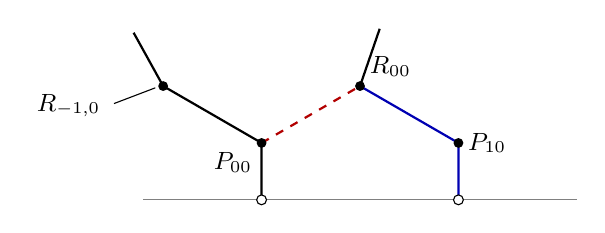
\begin{tikzpicture}[scale=2.5,font=\small]
\draw[gray](-.6,-.289)--(1.6,-.289);
\draw[thick](-.5,.289)--(0,0)--(0,-.289);
\draw[dashed,red!70!black,thick](0,0)--(.5,.289);
\draw[blue!70!black,thick](.5,.289)--(1,0)--(1,-.289);
\draw[thick](-.5,.289)--(-.65,.56);
\draw[thick](.5,.289)--(.6,.58);
\foreach \x/\y in {0/0,.5/.289,1/0,-.5/.289}{\fill(\x,\y)circle(.025);}
\foreach \x in {0,1}{\draw[fill=white](\x,-.289)circle(.025);}
\node[below left]at(0,0){$P_{00}$};
\node[above right]at(.5,.289){$R_{00}$};
\node[right]at(1,0){$P_{10}$};
\node[left]at(-.77,.19){$R_{-1,0}$};
\draw[thin](-.75,.20)--(-.54,.28);
\end{tikzpicture}
\caption{Separating the two branches at an internal minimum. When $P_{10}$ is absent, replace the dashed bond by the blue bond and start the second branch at the right port. When $P_{10}$ is already present, remove the two-bond initial segment through $R_{00}$ instead. The continuations drawn above are schematic.}\label{fig:minimum}
\end{figure}

First suppose there is one end. On the event $V\le r$, its last renewal is at height at most $C(1+r)$. After removing its no-renewal remainder and dropping the restriction on that remainder's final vertex, the mass is at most
\[
 C U_N\sum_{h\le C(1+r)}B_h
       \le C'(1+r)^{3/4}U_N
       \le C''(1+r)^{3/4}U_N^2,
\]
using \eqref{eq:strip-input} and $U_N\ge\rho/2$.

Now suppose there are two ends. Remove their no-renewal remainders and fix those remainders up to translation. Their $z$-weights will be summed at the end. Discard all avoidance constraints involving a remainder and the remaining total-length restriction, but retain the resulting $O(N^2)$ cap on bridge heights and piece counts. Drop the bridge damping factors $e^{-L_i/N}\le1$, so their weights are critical and the third input applies. The remaining two bridges have adjacent starts. If both are nonempty, they remain disjoint throughout the common height range. Put their heights and counts into dyadic bins and use the input's notation. If $a=\min(\kappa_1,\kappa_2)$ and $M=\max(\kappa_1,\kappa_2)$, then $K_i\ge\kappa_i$ gives
\[
 F=\frac{\kappa_1^2\kappa_2^2}{K_1K_2a}\le M.
\]
If $M$ is bounded by the fixed count threshold of Proposition~\ref{R:geo:chain}, the bound without a concentration test is already $O_\varepsilon(N^\varepsilon)$ and suffices. Otherwise choose a bridge $i$ attaining $M$, with a fixed tie rule; its count is large enough to supply the reserved group. In the integration for \eqref{eq:two-node-input}, fix the other bridge, the local records and the increments of bridge $i$ outside its reserved group; the two remainder shapes are already fixed. If $h_j$ is the other bridge's height, the endpoint-height condition restricts the total height of bridge $i$ to
\[
 [h_j+b-r-C_0,\ h_j+b+r+C_0],
\]
where $C_0$ bounds the endpoint-height changes and $b$ is determined by the two remainder endpoint heights and the fixed local records. Subtracting the fixed height of the other increments gives an interval of the same size for the reserved group's height. Its horizontal displacement is still summed over, so this is precisely the permitted concentration test. Thus \eqref{eq:two-node-input} bounds the mass in this pair of bins by
\[
 C_\varepsilon N^\varepsilon M
       \min\{1,(1+r)M^{-4/3}\}
       \le C_\varepsilon N^\varepsilon(1+r)^{3/4}.
\]
The last inequality follows by considering $M\le(1+r)^{3/4}$ and its complement. If only one bridge is nonempty, its factor $\kappa^2/K\le\kappa$ gives the same estimate: bounded $\kappa$ needs no concentration test, and larger $\kappa$ permits the calculation above. If neither is nonempty, the mass is at most one before the remainder weights are restored.

Because $L\le N^2$, there are only $O((\log N)^4)$ pairs of height/count bins. Choose the exponent slack in the geometric input smaller than the desired $\varepsilon$ and absorb this factor. Summing the two fixed remainder weights gives $U_N^2$. Their translations were determined by the bridge tips; no free placement factor is introduced. This proves the bound.
\end{proof}

\subsection{Length, spatial scale and moments}
\begin{samepage}
\begin{theorem}[Unrestricted thermal law]\label{thm:thermal}\label{R:thermal:law}
Choose an ordinary plane honeycomb walk from a fixed vertex with probability proportional to $(\rho e^{-1/N})^n$, where $n$ is its edge length. For every $\xi>0$, its vertex length $L$, endpoint distance $A$ and diameter $D$ satisfy
\[
 \Pp_N\{N^{1-\xi}\le L\le N^{1+\xi},\quad
 N^{3/4-\xi}\le A\le D\le N^{3/4+\xi}\}\longrightarrow1.
\]
For every fixed $p>0$,
\[
 \E_N L^p=N^{p+o(1)},\qquad
 \E_N A^p=N^{3p/4+o(1)},\qquad
 \E_N D^p=N^{3p/4+o(1)}.
\]
\end{theorem}
\end{samepage}
\begin{proof}
We use the equivalent vertex-weighted translation-class law. First record a consequence of \eqref{eq:count-input}. For each $\epsilon>0$, $p\ge0$ and $B>0$,
\begin{equation}\label{eq:damped-tail}
 \sum_{m>N^{1+\epsilon}}m^p a_m e^{-m/N}=O_{\epsilon,p,B}(N^{-B}).
\end{equation}
Indeed choose $0<\delta<\epsilon/(1+\epsilon)$. Uniformly for $m\ge N^{1+\epsilon}$, one has $m^\delta\le m/(2N)$ for all large $N$. The summands are then at most $C_\delta m^p e^{-m/(2N)}$, whose sum has faster than polynomial decay. In particular, paths with $L>N^2$ have negligible absolute mass and negligible mass after multiplication by any fixed length power. Since Lemma~\ref{lem:denominator} gives $Z_N\ge c/q_N$, this remains true after normalization.

Take $r=N^{3/4-\delta}$ with fixed $0<\delta<3/4$. Lemmas~\ref{lem:denominator} and~\ref{lem:twoends} give
\[
 \Pp_N\{V\le r,\ L\le N^2\}
       \le C_\varepsilon N^\varepsilon q_N(1+r)^{3/4}
       =N^{\varepsilon-3\delta/4+o(1)}.
\]
Choose $\varepsilon<3\delta/4$ and add the tail just discarded. It follows that $V\ge N^{3/4-\delta}$ with probability tending to one. After slightly decreasing the exponent tolerance to absorb $d_0$, the same lower bound holds for $A$.

We next obtain the upper spatial estimate from the absolute fast-path bound. Fix $\xi>0$. Choose small positive $\epsilon,\eta$ such that
\[
 (1+\epsilon)(3/4+\eta)<3/4+\xi.
\]
For lengths $m\le N^{1/2}$, the deterministic estimate $D\le Cm$ already gives the desired upper bound for large $N$. For $N^{1/2}<m\le N^{1+\epsilon}$, any violation of $D\le N^{3/4+\xi}$ implies $D>m^{3/4+\eta}$. Summing \eqref{eq:fast-input} over this range gives a faster than polynomially small absolute mass. Lengths above $N^{1+\epsilon}$ are handled by \eqref{eq:damped-tail}. Division by $Z_N$ proves the upper spatial assertion.

The same argument gives the lower length estimate, rather than assuming it from the discount scale. Fix $0<\xi<1$, choose $\eta,\delta>0$ so small that
\[
 (1-\xi)(3/4+\eta)<3/4-\delta,
 \qquad \delta<1/4.
\]
On the typical event $A\ge N^{3/4-\delta}$, a walk of length $m\le N^{1/2}$ is impossible for large $N$. If instead $N^{1/2}<m<N^{1-\xi}$, that endpoint event forces $D>m^{3/4+\eta}$, up to fixed unit factors absorbed by the strict inequality above. The summed exceptional mass is again negligible by \eqref{eq:fast-input}. Hence $L\ge N^{1-\xi}$ with high probability. The upper length bound follows from \eqref{eq:damped-tail}. Larger tolerances follow from smaller ones.

For moments, the lower probability estimates give the respective lower exponents. For the upper length moment, restrict to $L\le N^{1+\epsilon}$ and use \eqref{eq:damped-tail} on its complement:
\[
 \E_N L^p\le N^{p(1+\epsilon)}+o(1).
\]
For the spatial upper moments, repeat the fast-path split with the additional factor $D^p\le C_pL^p$. On the exceptional paths of polynomially large length, the factor is harmless in the sum of \eqref{eq:fast-input}; on the damped long-length tail use \eqref{eq:damped-tail} with this $p$. The remaining paths obey $D\le N^{3/4+\xi}$, apart from the deterministic short-length class. Thus
\[
 \E_N A^p\le\E_N D^p\le N^{p(3/4+\xi)}+o(1).
\]
Let the positive slacks decrease to zero. This completes the proof.
\end{proof}
The proof used the same irreducible law as exact-length conditioning, but a different denominator. It required no estimate of $U_N$, no local renewal mass at length $N$, and no inversion of a density-one statement. The part shared with exact conditioning is the renewal model and its increment estimates; the geometric recovery and two-end smoothing are the additional work needed for the unrestricted thermal law.
